\chapter{\label{method}Extensions and Innovation}

The system we have considered is an ideal system. Classically, what we have modelled is a dissipationless system that will continue its motion without a loss in energy. But all real experiments have a dissipative element in the system and in this case, it is the damping due to the springs, which are not ideal. Upon observing the readings, it was obvious to us that there is a damping present due to the rubber band connecting the two scales and due to the nature of the scales which will also lose energy over time. But this dissipation is not obvious enough to be observable in the dataset that we collect from the oscilloscope. Its observation takes at least 10 seconds using the oscilloscope under normal conditions. To study the damping effect of our 'springs', we attached one more rubber band to one of the scales using a rigid support. The system essentially remains the same as before with just the effective spring constant changing for one of the springs. But now, the damping is significant enough to be taken into account. The modified equations for the coupled oscillator with damping become
$$F_1=-k_1x_1+K(x_2-x_1)=m_1\ddot{x}_{1}$$
$$F_1=-(k_2+k_3)x_2+K(x_2-x_1)-k_v\frac{d ^\alpha x_2}{dt^\alpha}=m_2\ddot{x}_{2}$$
$\alpha$ and $k_v$ are parameters that cannot be determined theoretically. An approximate analytic solution for a single mass oscillator exists only for small $\frac{k_v}{m_2}$. It can give us an idea of the form of damping caused due to the rubber band\footnote{Yan Huang et al 2020 IOP Conf. Ser.: Mater. Sci. Eng. 782 022093}.
\[ m \frac{d^{2} x}{d t^{2}}+k_{\mathrm{v}} \frac{d^{\alpha} x}{d t^{\alpha}}+k x=0 \]
\[\frac{d^{2} x}{d t^{2}}+2 \beta \frac{d^{\alpha} x}{d t^{\alpha}}+\omega_{0}^{2} x=C\]Where, \( 2 \beta=\frac{\mathrm{k}_{\mathrm{v}}}{\mathrm{m}}, \omega_{0}^{2}=\frac{\mathrm{k}}{\mathrm{m}} \), and the initial condition is set to be \( x(0)=x_{0}, \dot{x}(0)=0 \).
For the case of \( 0<\beta<1 \), when \( \beta \) can be regarded as a small parameter, the approximate analytical solution of the equation(3) can be obtained by means of the average method as follows\[x(t)=x_{0} e^{-\beta \omega_{0}^{\alpha-1} \sin \frac{\alpha \pi}{2} t} \cos \left[\left(\omega_{0}+\beta \omega_{0}^{\alpha-1} \cos \frac{\alpha \pi}{2}\right) t\right]\]The corresponding solution of equation (1) is\[x(t)=x_{0} e^{-\frac{1}{2 m} k_{v}\left(\sqrt{\frac{k}{m}}\right)^{\alpha-1} \sin \frac{\alpha \pi}{2} t} \cos \left\{\left[\sqrt{\frac{k}{m}}+\frac{1}{2 m} k_{v}\left(\sqrt{\frac{k}{m}}\right)^{\alpha-1} \cos \frac{\alpha \pi}{2} \mid t\right\}\right.\]
\[\begin{aligned}\Delta & =\frac{1}{2 m} k_{\mathrm{v}}\left(\sqrt{\frac{k}{m}}\right)^{\alpha-1} \sin \frac{\alpha \pi}{2} \\\omega_{\mathrm{v}} & =\frac{1}{2 m} k_{\mathrm{v}}\left(\sqrt{\frac{k}{m}}\right)^{\alpha-1} \cos \frac{\alpha \tau}{2}\end{aligned}\]The equation (5) can be changed into\[x(t)=x_{0} e^{-\Delta t} \cos \left[\left(\omega_{0}+\omega_{\mathrm{v}}\right) t\right]\]

This equation is a cosine simple harmonic oscillator term multiplied by an exponential damping term. The system that we are studying in our experiment is a coupled oscillator and it does not have a simple cosine dependence for the harmonic oscillation part and instead is a linear combination of two normal modes hence, beats can emerge because the two oscillators are connected and their natural oscillating frequencies are of the same order of magnitude. Since these beats have a more complicated solution, we cannot directly say how the damped solution will look. But, we know that what the rubber band is essentially doing is dissipating energy. We know that the energy of an oscillator is directly proportional to the square of the amplitude. Hence, we know that if energy is dissipated, the amplitude will decrease and we saw that for a single oscillator. For the coupled oscillator, we propose that we will see an exponential decay in the amplitude of oscillation in the beats and a part of our experiment works towards finding out this decay term. What we have to do is to find the amplitude in every single beat unit and plot it as a function of time. If this turns out to be an exponential decay then we have verified our hypothesis. This is because the total energy of the system is directly proportional to the sum of squares of individual oscillator amplitudes.
Since beats have the form 
\[\cos \left(\omega_{1} t\right)+\cos \left(\omega_{2} t\right)=2 \cos \left(\frac{\omega_{1}+\omega_{2}}{2} t\right) \cos \left(\frac{\omega_{1}-\omega_{2}}{2} t\right)\]
We expect our final curve to look like 
\[a(t)=e^{-\Delta t}\left\{  2 \cos \left(\frac{\omega_{1}+\omega_{2}}{2} t\right) \cos \left(\frac{\omega_{1}-\omega_{2}}{2} t\right)\right\}\]
Experimentally, we only need to obtain the maximum values of the cosine part to get an exponential decaying term.

\section{Observations}
Here we have tabulated the decay constants we found for different masses after doing curve-fitting, along with the plots.

\begin{figure}[H]
	\centering
	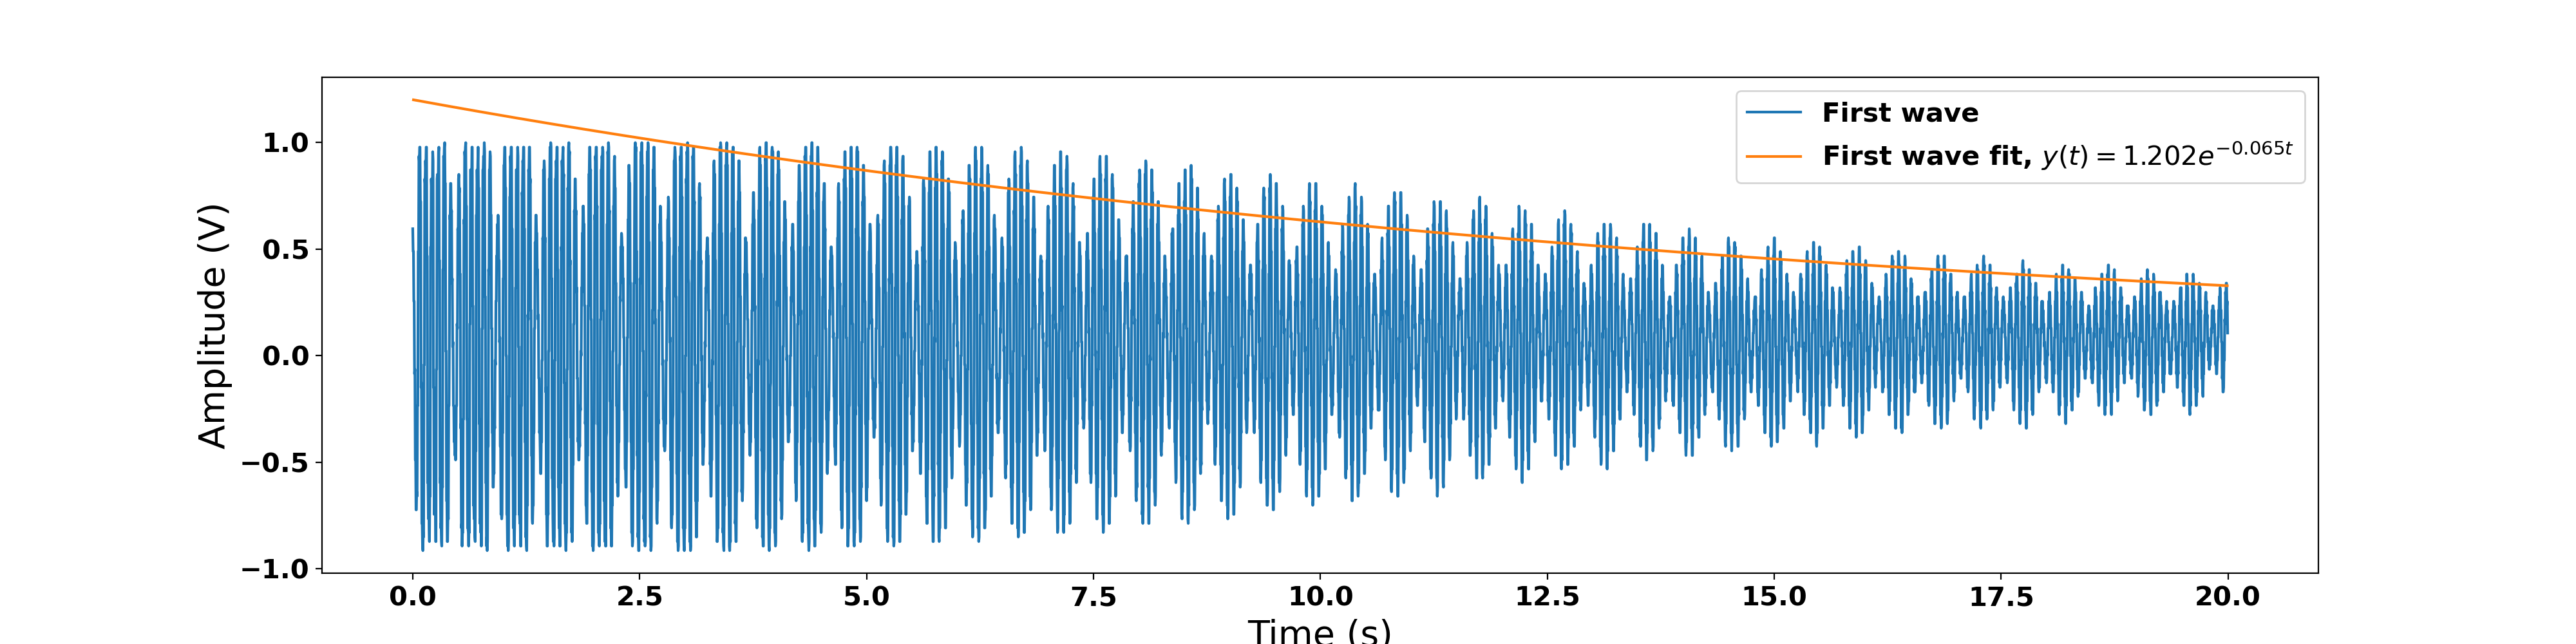
\includegraphics[scale=0.35]{03_1.png}
	\caption{Decaying amplitude due to daming by the rubber band attached to the mounted aluminium beam, fitted with the it's decay law}
	\label{fig:mb-fe-0}
\end{figure}

\begin{figure}[H]
	\centering
	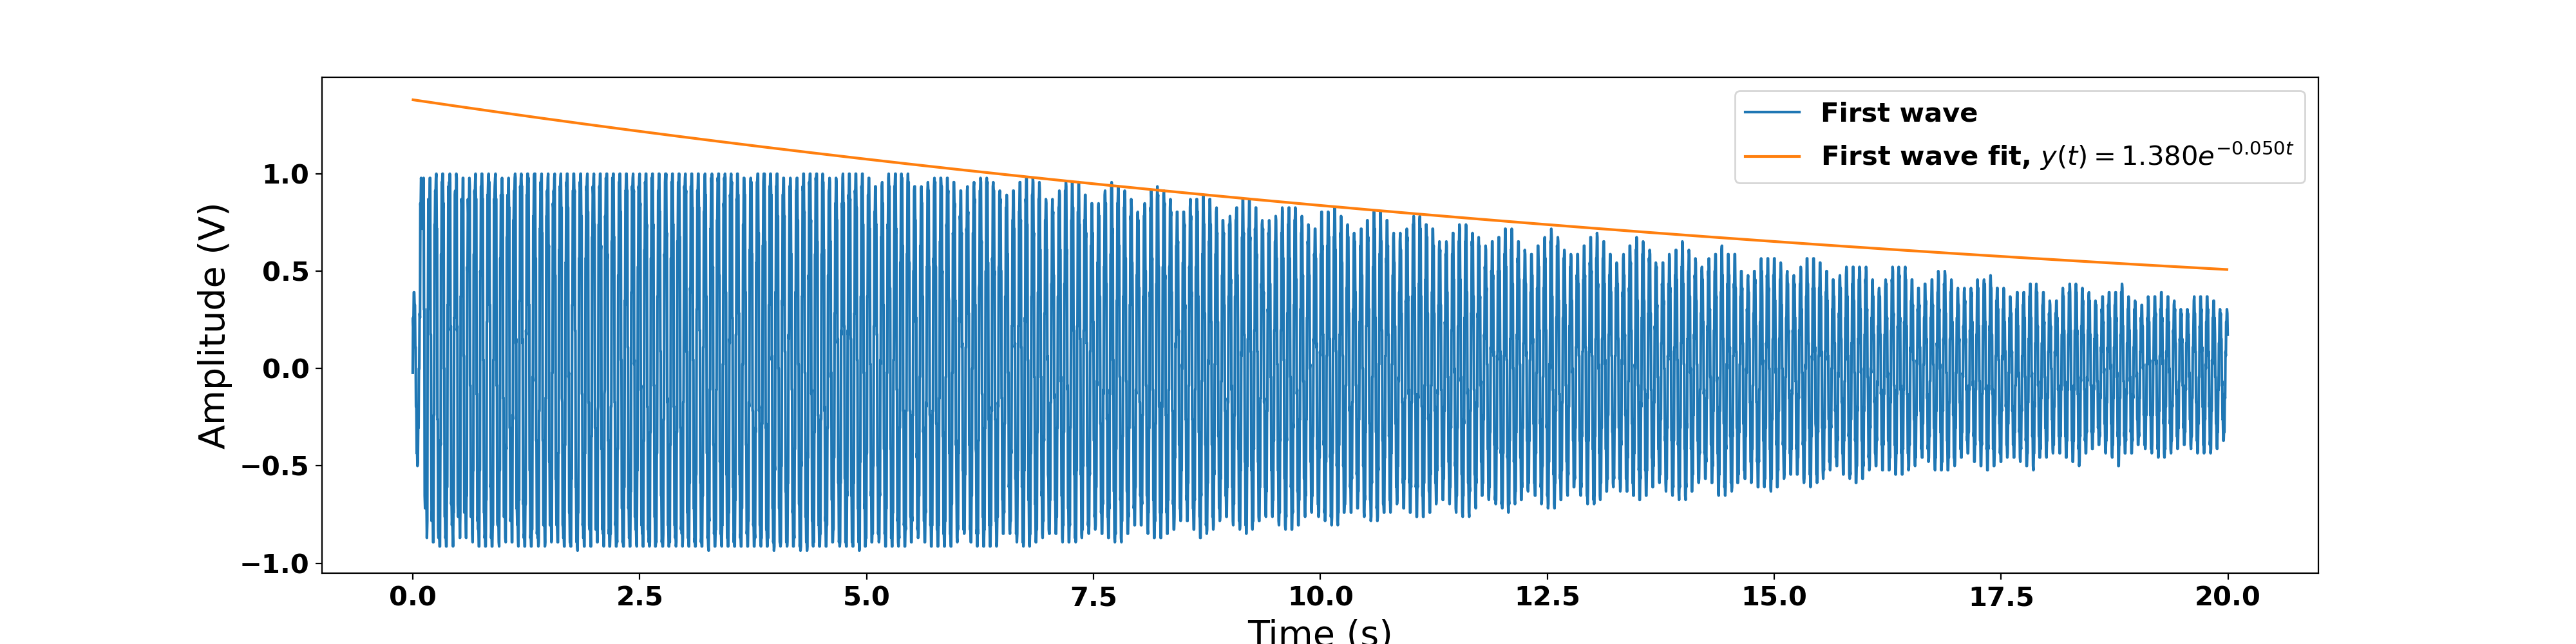
\includegraphics[scale=0.35]{04_1.png}
	\caption{Decaying amplitude due to daming by the rubber band attached to the mounted aluminium beam, fitted with the it's decay law}
	\label{fig:mb-fe-0}
\end{figure}

\begin{figure}[H]
	\centering
	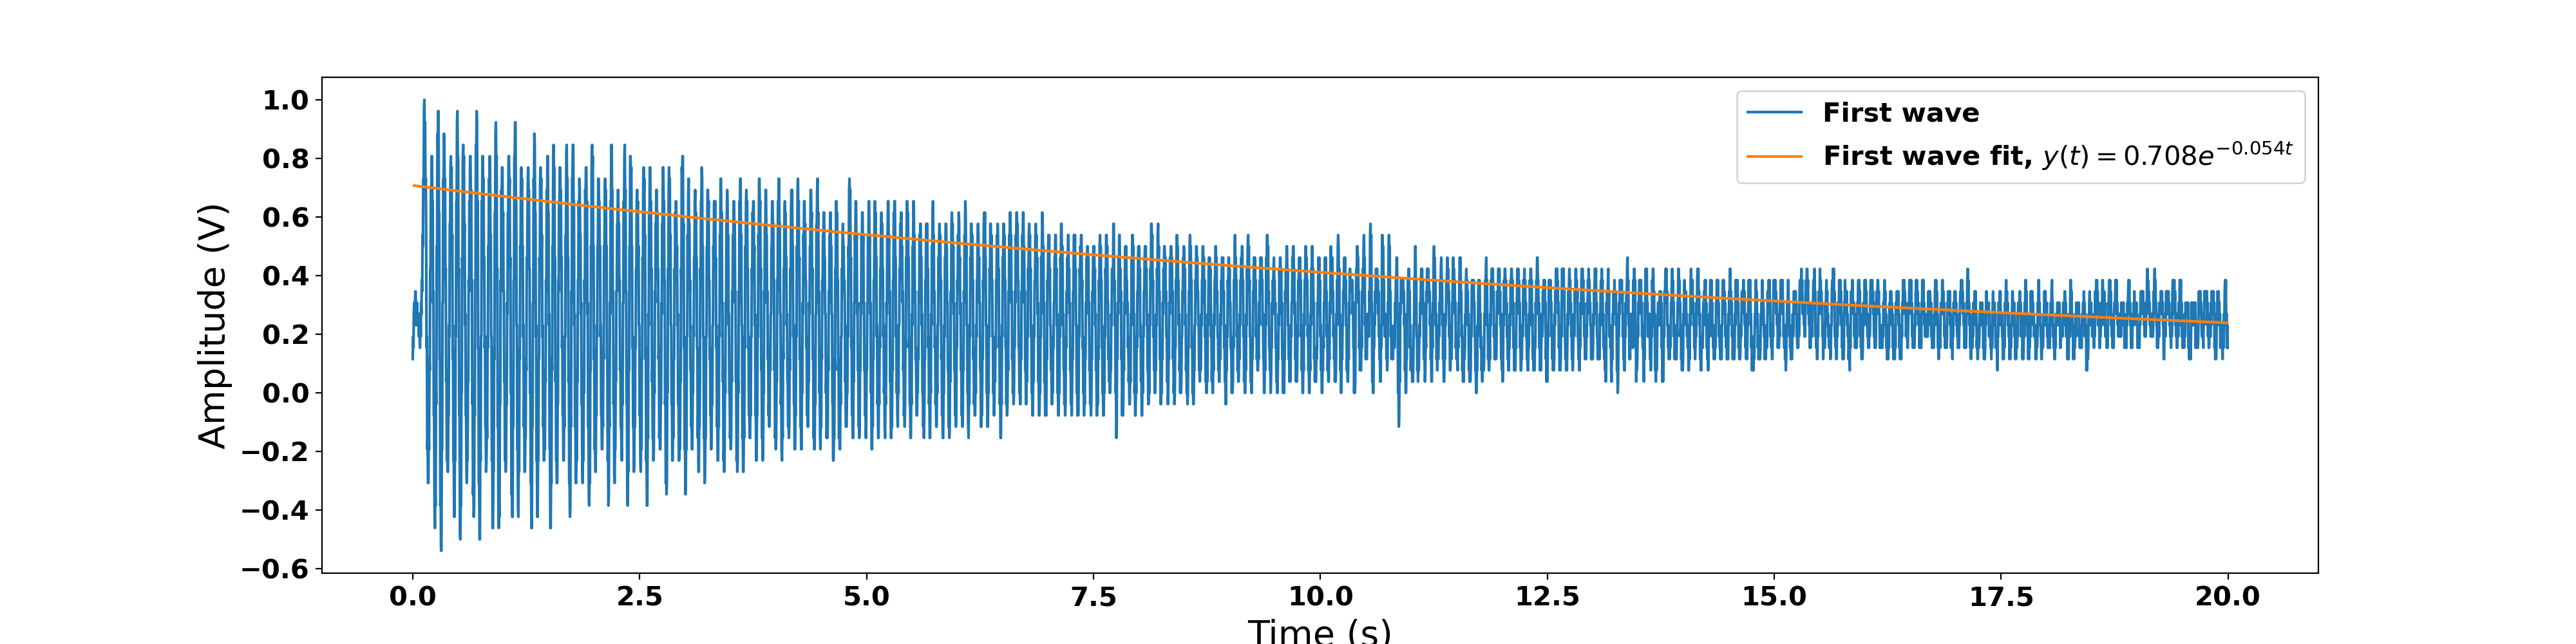
\includegraphics[scale=0.35]{05_1.png}
	\caption{Decaying amplitude due to daming by the rubber band attached to the mounted aluminium beam, fitted with the it's decay law}
	\label{fig:mb-fe-0}
\end{figure}
\begin{figure}[H]
	\centering
	\includegraphics[scale=0.35]{16_1.png}
	\caption{Decaying amplitude due to daming by the rubber band attached to the mounted aluminium beam, fitted with the it's decay law}
	\label{fig:mb-fe-0}
\end{figure}
\begin{figure}[H]
	\centering
	\includegraphics[scale=0.35]{17_1.png}
	\caption{Decaying amplitude due to daming by the rubber band attached to the mounted aluminium beam, fitted with the it's decay law}
	\label{fig:mb-fe-0}
\end{figure}
\setcounter{equation}{0}
\setcounter{table}{0}
\setcounter{figure}{0}